\section{Theoretical part}

\subsection{Domain Name System}
\subsubsection{DNS provisions}
The DNS system ensures fault tolerance on a packet level through UDP, which
wraps the segments in a header containing a checksum. On a system level fault
tolerance is ensured because the system is designed as a distributed
architecture, making sure that there are no central points of failure. Both of
these techniques also ensure scalability by making making DNS have stateless
connections and spreading requests out over a large amount of servers.
Efficiency is then also ensured because UDP has a very low overhead compared to
TCP, and one may query servers that are close.

\subsubsection{DNS lookup and format}
\begin{description}
    \item[Part 1:] The CNAME record allows a server to be known through several
        aliases, such as a web-server being named www.domain.tld and a ftp
        service on the same server being named ftp.domain.tld. It may also be
        used to load-balance requests by returning CNAME records for a domain
        that redirect users to multiple servers, maybe even servers closer to
        the user. Multiple CNAME records violates the standard,\footnote{BIND 9
            Administrator Manual,
        page 62} but is widely used in practice.
    \item[Part 2:] Iterative lookups work by the root and TLD servers
        delegating further lookups to the requesting party, instead of
        performing them themselves.
        This means that the local DNS server (the one that a client is asking),
        will ask another server and receive an answer, then acting on the
        information in that answer to fulfill the request (by further lookups).
        In a recursive lookup the server that is being asked is the one that
        queries further servers for more detailed information, and it will only
        return once it has an authoritative answer.

        Iterative lookups place less strain on the DNS network, because only
        the local DNS server has to maintain state about the request that is
        being answered. This enables the system to scale better. The caches of
        the local DNS server will also be filled with information on
        authoritative and TLD servers, cutting off the root level and speeding up
        requests.

        %TODO: When and why do we want recursive lookups? Is it something about
        %using it to fill caches?
    %TODO: See figure 2.21
    \item[Part 3:] The query to \url{groveshark.com} is answered the follwoing
        way. An important fact to note is that root servers are always
        iterative servers.
        \begin{enumerate}
            \item DikuStudent sends the query 'what is the IP address of
                \texttt{grooveshark.com}' to locally configured DNS server
                \texttt{ns2.censurfridns.dk} at 89.104.194.142.
            \item \texttt{ns2.censurfridns.dk} looks up
                \texttt{grooveshark.com} in local cache, but nothing is found.
            \item \texttt{ns2.censurfridns.dk} sends query to a root-server
                (eg. \texttt{a.root-servers.net} at ip 198.41.0.4) for the
                IP of \texttt{grooveshark.com}
            \item The root-server throws the warning, "recursion requested but
                not available", and replies with a referral to the TLD servers
                for .com (\texttt{[a-m].gtld-servers.net})
                \begin{lstlisting}
;; ->>HEADER<<- opcode: QUERY, status: NOERROR, id: 26454
;; flags: qr rd; QUERY: 1, ANSWER: 0, AUTHORITY: 13, ADDITIONAL: 16
;; WARNING: recursion requested but not available

;; OPT PSEUDOSECTION:
; EDNS: version: 0, flags:; udp: 512
;; QUESTION SECTION:
;groveshark.com.            IN  A

;; AUTHORITY SECTION:
com.            172800  IN  NS  a.gtld-servers.net.
com.            172800  IN  NS  b.gtld-servers.net.
com.            172800  IN  NS  c.gtld-servers.net.
com.            172800  IN  NS  d.gtld-servers.net.
com.            172800  IN  NS  e.gtld-servers.net.
com.            172800  IN  NS  f.gtld-servers.net.
com.            172800  IN  NS  g.gtld-servers.net.
com.            172800  IN  NS  h.gtld-servers.net.
com.            172800  IN  NS  i.gtld-servers.net.
com.            172800  IN  NS  j.gtld-servers.net.
com.            172800  IN  NS  k.gtld-servers.net.
com.            172800  IN  NS  l.gtld-servers.net.
com.            172800  IN  NS  m.gtld-servers.net.

;; ADDITIONAL SECTION:
a.gtld-servers.net. 172800  IN  AAAA    2001:503:a83e::2:30
a.gtld-servers.net. 172800  IN  A   192.5.6.30
b.gtld-servers.net. 172800  IN  AAAA    2001:503:231d::2:30
b.gtld-servers.net. 172800  IN  A   192.33.14.30
c.gtld-servers.net. 172800  IN  A   192.26.92.30
d.gtld-servers.net. 172800  IN  A   192.31.80.30
e.gtld-servers.net. 172800  IN  A   192.12.94.30
f.gtld-servers.net. 172800  IN  A   192.35.51.30
g.gtld-servers.net. 172800  IN  A   192.42.93.30
h.gtld-servers.net. 172800  IN  A   192.54.112.30
i.gtld-servers.net. 172800  IN  A   192.43.172.30
j.gtld-servers.net. 172800  IN  A   192.48.79.30
k.gtld-servers.net. 172800  IN  A   192.52.178.30
l.gtld-servers.net. 172800  IN  A   192.41.162.30
m.gtld-servers.net. 172800  IN  A   192.55.83.30

;; Query time: 319 msec
;; SERVER: 198.41.0.4#53(198.41.0.4)
;; WHEN: Sun May 12 18:36:07 2013
;; MSG SIZE  rcvd: 531

                \end{lstlisting}
            \item \texttt{ns2.censurfridns.dk } sends query 'what is the IP
                address of \texttt{groveshark.com}' to one of the .com TLD servers (eg
                \texttt{m.gtld-servers.net}).
            \item The TLD server throws the warning, "recursion requested but
                not available", and replies with a referral to the name servers
                for \texttt{groveshark.com}
                (\texttt{ns51.1and1.com} and \texttt{ns52.1and1.com})
                \begin{lstlisting}
;; ->>HEADER<<- opcode: QUERY, status: NOERROR, id: 25222
;; flags: qr rd; QUERY: 1, ANSWER: 0, AUTHORITY: 2, ADDITIONAL: 3
;; WARNING: recursion requested but not available

;; OPT PSEUDOSECTION:
; EDNS: version: 0, flags:; udp: 4096
;; QUESTION SECTION:
;groveshark.com.            IN  A

;; AUTHORITY SECTION:
groveshark.com.     172800  IN  NS  ns51.1and1.com.
groveshark.com.     172800  IN  NS  ns52.1and1.com.

;; ADDITIONAL SECTION:
ns51.1and1.com.     172800  IN  A   217.160.80.164
ns52.1and1.com.     172800  IN  A   217.160.81.164

;; Query time: 162 msec
;; SERVER: 192.42.93.30#53(192.42.93.30)
;; WHEN: Sun May 12 18:37:32 2013
;; MSG SIZE  rcvd: 119
                \end{lstlisting}
            \item \texttt{ns2.censurfridns.dk } sends query 'what is the IP
                address of groveshark.com' to one of the nameservers (eg.
                \texttt{ns52.1and1.com}).
            \item Zone file defines the A record for \texttt{groveshark.com}
                \begin{lstlisting}
;; ->>HEADER<<- opcode: QUERY, status: NOERROR, id: 41882
;; flags: qr aa rd; QUERY: 1, ANSWER: 1, AUTHORITY: 0, ADDITIONAL: 1
;; WARNING: recursion requested but not available

;; OPT PSEUDOSECTION:
; EDNS: version: 0, flags:; udp: 2800
;; QUESTION SECTION:
;groveshark.com.            IN  A

;; ANSWER SECTION:
groveshark.com.     10800   IN  A   74.208.29.191

;; Query time: 24 msec
;; SERVER: 217.160.81.164#53(217.160.81.164)
;; WHEN: Sun May 12 18:38:15 2013
;; MSG SIZE  rcvd: 59
                \end{lstlisting}
            \item Send response \texttt{groveshark.com} has A record
                74.208.29.191, to DikuStudent.
        \end{enumerate}
        Below is a illustration of the queries made. If the root and tld server
        had accepted the recursive request, then the root server would have
        asked, then tld, who would have asked the authority dns server.
        \begin{figure}[!h]
        \centering
        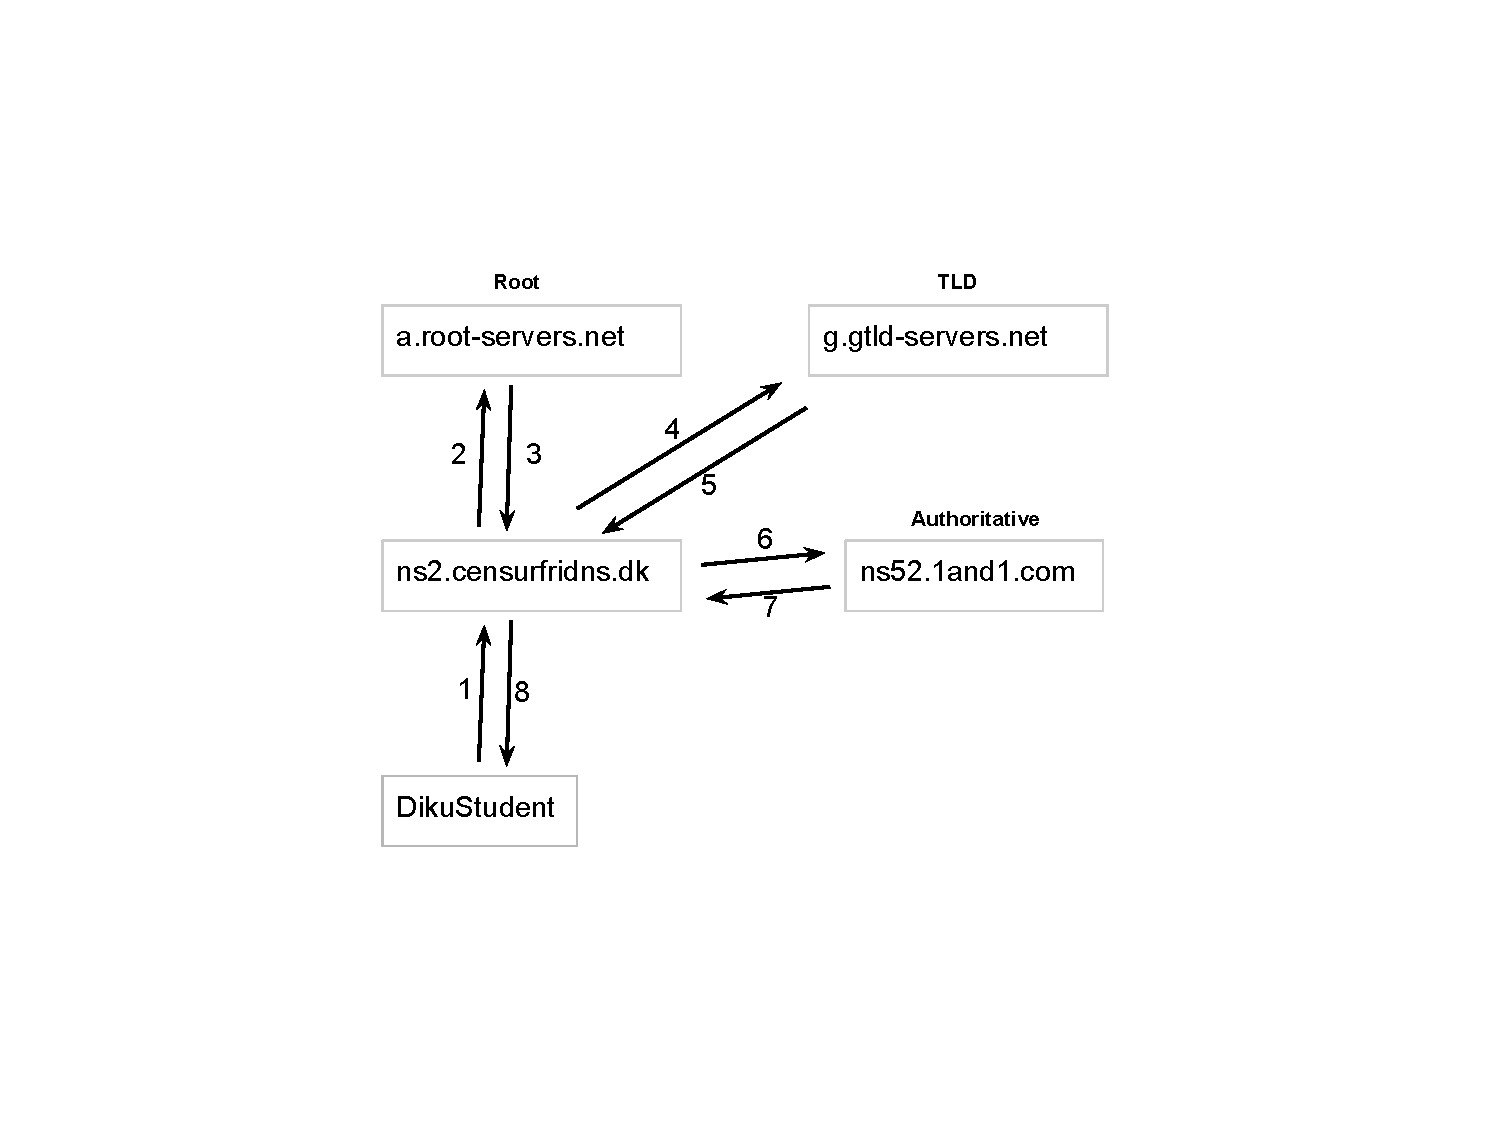
\includegraphics[trim = 55mm 30mm 55mm 30mm, clip, width=10cm]{112p3-pic}
        \caption{Resolving groveshark.com}
        \end{figure}

\end{description}

\subsection{Transport protocols}
\subsubsection{TCP reliability and utilization}
\begin{description}
    \item[Part 1:] The 3-way handshake ensures that both sides have received
        the starting segment number of the other side. If the final ACK is not
        sendt, the server cannot be certain that it's starting segment number
        has actually reached the client. If we wish to be sure that the
        connection is correctly initialized on both sides we must therefore use
        all parts of the 3-way-handshake.
    \item[Part 2:] TCP facilitates a full-duplex connection by making the ACK a
        field in the header of segments, thus allowing mixing an answer to a
        segment with a new data segment to be delivered to the other side. The
        setup also initializes the link in both directions, so both sides are
        ready to send to each other.
\end{description}

\subsubsection{Reliability vs overhead}
\begin{description}
    \item[Part 1:] TCP adds overhead both in the header (being approx. 20 bytes
        in size, compared to 8 bytes for UDP), and by requiring that all
        segments are acknowledged and optionally re-sent. It must also
        negotiate segment numbers before starting to transmit data, while UDP
        starts blasting data immediately.
    \item[Part 2:] The TCP protocol uses a sequence number to identify each
        byte of data, this number reflect the order of the bytes sent and is
        used to ensure reliability of the data, the initial sequence number is
        chosen at random, and simply incremented after each byte sent. When the
        reciever receives a TCP segment, he checks that the sequence number
        match's his acknowledgment number(the sequence number he expected
        next), if it is a match, he increment the acknowledgment number by 1 and
        put it in the header of the next TCP segment he sends back, if the
        sequence number does not match, he will not increace the acknowledgment
        number, but still sending the it back (and in that way telling the
        sender, ``Hayo, I need from segmentnumber x and up'').
\end{description}


\subsubsection{Use of transport protocols}
\begin{description}
    \item[DNS part 1:] DNS employs the UDP transport protocol. This is because it has a low overhead, does not require
        the connections to negotiate before sending data, or keep state on a connection. The result of this is that the DNS
        protocol scales much better than if it was sent over a stateful transport protocol like TCP. %TODO: More?
    \item[DNS part 2:] The use of TCP for DNS could have eliminated cache-poisoning attacks, because an attacker would then have
        to brute-force the 32-bit sequence number in the TCP packet in addition to the 16-bit DNS identification number.
        Such an attack would clealy be infeasible.

        The result of a cache-poisoning is that a DNS server caches an incorrect and malicious response, leading to malicious redirects
        of the requests. The attack may then be spread further by legitimate requests to the poisoned server, that are then cached in
        other servers. As an example one could attempt to poison the DNS server of a Danish ISP, redirecting all requests for common banks
        to a compromised server. This server could then infect users or steal their credentials. One might also be able to redirect
        the domains used to serve the NemID-applet, instead sending a compromised version to browsers.
    \item[HTTP part 1:] The minimum number of packets is 3 for the handshake (where the last one can hold the request data because
        of the large MTU), 2 for the server ACK with corresponding data and the client ACK, and 4 for the closing of the connection.
        This results in a minimal number of 9 packets from a TCP perspective.
    \item[HTTP part 2:] Only 1/9 of the packets used for the connection actually transmit data. The justification for using
        TCP despite of this overhead is the fact that it provides the reliability needed by HTTP (as discussed in the next part), and
        that it allows for keeping connections open and thus reducing the setup overhead.
    \item[HTTP part 3:] The choice of UDP as a transport protocol for HTTP would be poor, because the guarantees provided by
        TCP are needed for HTTP transmissions. The use of HTTP does not allow for packets to be completely dropped (HTTP is not
        loss-tolerant), and the data stream must be presented in-order for the documents to make sense. In addition to this the
        HTTP protocol is naturally structured such that it fits the TCP model well, by defining a stream of requests and responses.
\end{description}

\subsection{TCP: Principles and practice}
% Specify the point of view, is it from the client's or server's side (or both)?
\subsubsection{TCP headers}
\begin{description}
    \item[Part 1.1:] The purpose of the RST bit is to inform the sender of a segment that it's destination IP or port was
        incorrect, such that it will stop sending further segments or stop expecting a connection to be set up. A TCP stack
        may return a RST packet if you attempt to send a SYN packet with a destination port that is not listening.
    \item[Part 1.2:] The sequence number header refers to the byte-stream number of the first byte in the sent segment. The
        acknowledgement number header refers to the segment number of the next expected byte to be received. The acknowledgement
        number header that is being sent in one direction is the sequence number of the next byte that is expected to be received.
    \item[Part 1.3:] The purpose of the window is to enable flow control of TCP streams, such that a receiver is not overwhelmed
        by data. A positive window size indicates that the sender may continue to send data, as there is room in the receive buffer
        to store it.
    \item[Part 1.4:] If the window size of the receiver is 0 the sender is required to send segments of size 1, such
        that it may receive an ACK with an updated window size. If this was not the case then the sender might have been
        permanently blocked from sending, even though the window size of the receiver changed.
    \item[Part 2:] The sending of data in the third step (the ACK) of the 3-way-handshake is possible because the initial
        sequence numbers have already been correctly exchanged at that point. %TODO: More?
    \item[Part 3:] Below is the diagram.
        \begin{figure}[!h]
        \centering
        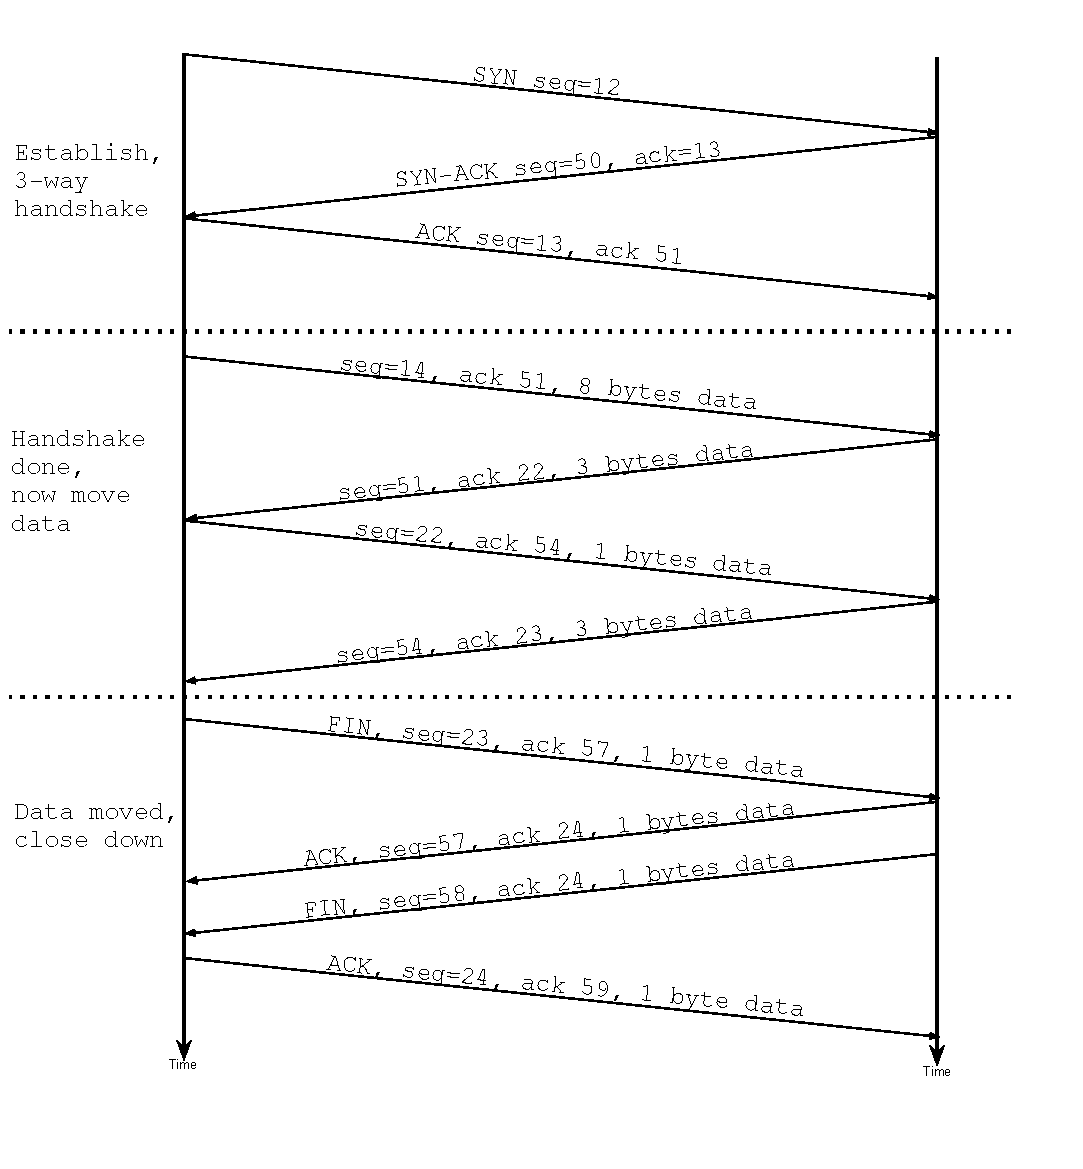
\includegraphics[width=10cm]{131p3-pic}
        \caption{TCP diagram}
        \end{figure}
\end{description}

\subsubsection{High performance TCP}
\begin{description}
    \item[Part 1:] The maximum possible number in receive window header is
        $2^{16}-1 = 65535$. This means that the throughput in one direction is
        limited to \[\frac{65525}{RTT} \text{ B/msec}\] %TODO: Rewrite?
    \item[Part 2:] Ignoring the overhead of TCP packet headers it would take a
        100Mb/s connection \[ \frac{65535 * 8 \text{ bits}}{100 * 10^{6} \text{
        bits/sec}} = 5.243 \text{ milliseconds} \] to send enough bytes to fill
        the receive window. We must therefore have $RTT \leq 5.243 \text{
        milliseconds}$ to fully utilize the connection.
    \item[Part 3:] If the roundtrip time is 72, then - in one direction - we
        can send $$72=\frac{8x}{10^8} \Rightarrow x = 9 \times 10^8$$ bytes.
        
        We are able to change the window size in two ways. (i) change the
        actual window size value, (ii) change the amount of bit shifting.
        
        We start by letting the window size be fixed at 65535 bytes and see
        that $9\times10^8$ is in between $65535*2^{13}=536862720$ and
        $65535*2^{14}=1073725440$, so we set the amount of bit-shifting to
        $14$. Now we just have to solve the following equaltion to obtain
        the value for the actual windows size field $$2^{14}x=9\times10^8 \Rightarrow x=\ceil{3515625/64} = 54932$$
        So for full utilization of the 100Mb connection, you set the 'Window
        Size' field to 54932 and the 'TCP Window Scale Option' to bit shift by
        14.
\end{description}

\subsubsection{Flow and Congestion control}
\begin{description}
    \item[Part 1:] Modern TCP implementation employ congestion control based on
        perceived network congestion. This is not network assisted, and works
        by measuring the ACK that are received to detect possible losses as a
        result of congestion. The traffic is then appropriately throttled.

    \item[Part 2:]
        During the initial data transfer phase the Slow Start algorithm is
        used, this algorithm continuously  increases transmission window size.

        If it happens that one or more packets are dropped doing Slow Start,
        then Congestion Avoidance is used to slow the transmission rate, by
        setting the transmission window size to half of the current window
        size.

        Slow Start is used in conjunction with Congestion Avoidance, and thus
        the data trasmission rate rises again over time instead of staying
        slow.

        If congestion is happenning on a later stage, the sender is forced into
        Slow Start again.

    \item[Part 3:] %TODO: Write at most 10 sentences
        
    \item[Part 4:]
    %How many ACKs should the sender receive before doing a fast retransmit?
    The sender should receive 4 ACKs without any packet arriving in between
    -- one ACK for previous package and 3 duplicates. Then it can do the fast
    retransmit.
    %What does the sender need to implement?
    The sender need to keep the content of non-ACK'ed packets as there may be a need to retransmit them.
    The sender must also keep track of the number of duplicate ACKs arriving. If this number reaches 3 before receiving any other packet, the sender must retransmit the packet following the duplicate ACK'ed packet.
    %What does the receiver need to implement?
    The receiver must keep track of the sequence number for next packet arriving to make a continuous stream (next expected packet). If a packet arrives that has a higher sequence number, an ACK is send containing the sequence number for the next expected packet. The receiver must keep track of these ``higher'' packets, so when the gap fills, it can report which sequence number it is ready to receive next.

\end{description}
